\documentclass{article}
\usepackage{hyperref}
\usepackage{graphicx} % Required for inserting images

\title{MVP}
\author{Automatic Project Detection And Tooling For Devs}
\date{}

\begin{document}
\maketitle

\section{User stories}

\begin{figure}[h]
    \centering
    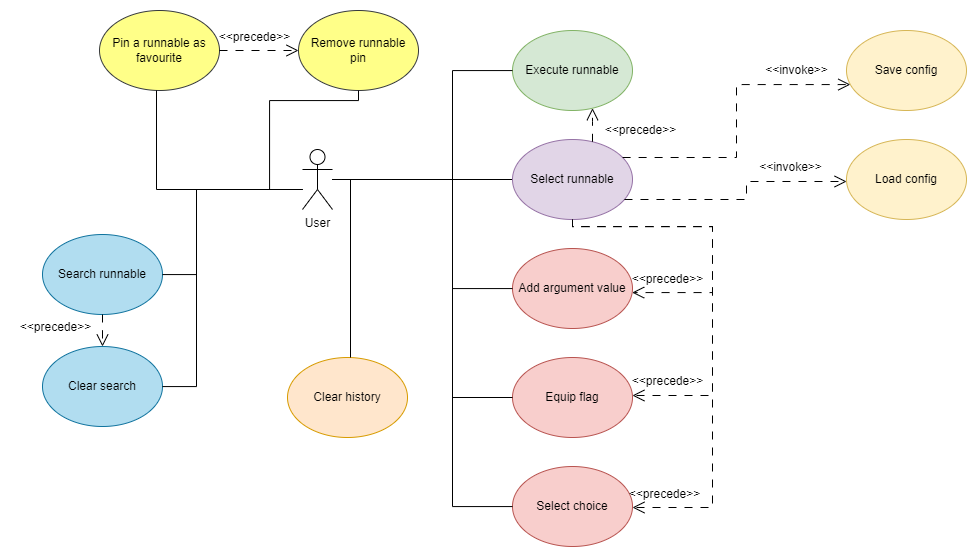
\includegraphics[width=1\linewidth]{img/use_case_diagram.drawio.png}
    \caption{Use case diagram}
    \label{fig:enter-label}
\end{figure}

\subsection{Select runnable}
\begin{itemize}
    \item \textbf{As a} user \textbf{I want} to select a runnable from the list of found runnables, \textbf{so that} I can configure its arguments.
\end{itemize}

\subsection{Add argument value}
\begin{itemize}
    \item \textbf{As a} user \textbf{I want} to give a value of an argument \textbf{so that} I can add it to the configuration.
\end{itemize}

\subsection{Equip flag}
\begin{itemize}
    \item \textbf{As a} user \textbf{I want} set a flag \textbf{so that} I can chose that the flag stores True or False.
\end{itemize}

\subsection{Select choices}
\begin{itemize}
    \item \textbf{As a} user \textbf{I want} to choose a value from the choices of the argument \textbf{so that} I can set it.
\end{itemize}

\subsection{Execute runnable}
\begin{itemize}
    \item \textbf{As a} user \textbf{I want} to execute a runnable \textbf{so that} I can press a button on the screen and the tool runs it with the given arguments.
\end{itemize}

\subsection{Save config}
\begin{itemize}
    \item \textbf{As a} user \textbf{I want} to save the configuration that I gave before \textbf{so that} the program saves it for me.
\end{itemize}

\subsection{Load config}
\begin{itemize}
    \item \textbf{As a} user \textbf{I want} to load the previously saved configuration for me \textbf{so that} the program loads for me.
\end{itemize}

\subsection{Clear history}
\begin{itemize}
    \item \textbf{As a} user \textbf{I want} to clear my configuration history \textbf{so that} the program deletes every configuration.
\end{itemize}

\subsection{Pin a runnable as favourite}
\begin{itemize}
    \item \textbf{As a} user \textbf{I want} to pin a runnable as favourite  \textbf{so that} the program highlights it.
\end{itemize}

\subsection{Remove runnable pin}
\begin{itemize}
    \item \textbf{As a} user \textbf{I want} remove a highlight from a runnable \textbf{so that} the program removes the highlight of the runnable.
\end{itemize}

\subsection{Search runnable}
\begin{itemize}
    \item \textbf{As a} user \textbf{I want} find a specified runnable \textbf{so that} I can search it from the list.
\end{itemize}

\subsection{Clear search}
\begin{itemize}
    \item \textbf{As a} user \textbf{I want} to clear the search history \textbf{so that} the program doesn't show the previously searched items.
\end{itemize}

\section{Prioritized user stories}

Prioritizing with the help of MoSCoW method.
\begin{itemize}
    \item M - Must have
    \item S - Should have
    \item C - Could have
    \item W - Won't have
\end{itemize}

\subsection{Must have user stories:}
\begin{itemize}
    \item Select runnable:
    \begin{itemize}
        \item Filters all runnables from the working direcoty.
        \item Collects all details of the runnables, such as description, name, and arguments. It also collects all information about the arguments.
        \item Full path to the runnable, that will be needed during execution.
    \end{itemize}
    \item Execute runnable
    \begin{itemize}
        \item Executing the runnable with using its full path and the appropriate compiler or interpreter.
        \item If information available of the values of the arguments, These must be used during execution.
    \end{itemize}
    \item Add argument
    \begin{itemize}
        \item This user story ensures that the user can provide a value for an argument as input.
    \end{itemize}
\end{itemize}

\subsection{Should have user stories}
\begin{itemize}
    \item Equip flag
    \begin{itemize}
        \item If the argument is a flag, user can switch whether it should store a true or false value.
    \end{itemize}
    \item Select choices
    \begin{itemize}
        \item If there are choices within the argument, the user should select one of them.
    \end{itemize}
    \item Save config
     \begin{itemize}
         \item Users are able to store their configurations.
     \end{itemize}
     \item Load config
     \begin{itemize}
         \item Users are able to load their previously saved configurations.
     \end{itemize}
     \item Clear history
     \begin{itemize}
         \item Users are able to delete their configurations.
     \end{itemize}
\end{itemize}

\subsection{Could have user stories}
\begin{itemize}
    \item Search runnable
    \begin{itemize}
        \item Users are able to search for specified runnables.
    \end{itemize}
    \item Clear search
    \begin{itemize}
        \item After searching users can delete their search history.
    \end{itemize}
\end{itemize}

\subsection{Won't have user stories }
\begin{itemize}
    \item Pin a runnable as favourite
    \begin{itemize}
        \item Users are able to pin runnables as favourite, and those will be highlighted.
    \end{itemize}
    \item Remove runnable pin
    \begin{itemize}
        \item Users are able to remove the highlight from a pinned runnable.
    \end{itemize}
\end{itemize}

\section{The content of the MVP}
MVP should contain these user stories, which have been prioritized.
\begin{itemize}
    \item Select runnable
    \item Add argument value
    \item Equip flag
    \item Select choices
    \item Execute runnable
    \item Save config
    \item Load config
    \item Clear history
    \item Search runnable
    \item Clear search
\end{itemize}

\section{MVP complete}
The complete MVP should contain these user stories below.
\begin{itemize}
    \item Select runnable
    \item Add argument value
    \item Equip flag
    \item Select choices
    \item Execute runnable
    \item Save config
    \item Load config
    \item Clear history
\end{itemize}

\section{MVP minimal}
None of this user stories can be taken out to avoid losing the point of MVP.
\begin{itemize}
    \item Select runnable
    \item Add argument value 
    \item Execute runnable
\end{itemize}

\section{MVP real}
The user stories below have the potential to be implemented realistically by the end of the project.
\begin{itemize}
    \item Select runnable
    \item Add argument value
    \item Equip flag
    \item Select choices
    \item Execute runnable
\end{itemize}

\section{KPI deffinition}

\section{KPI goal}

\end{document}